\section{Characterization} \label{sec:characterization}

In this section, the Omicron algorithm is characterized. First, the detection efficiency is evaluated. Then we measure how well signal parameters are estimated. To achive this, we consider colored Gaussian noise, the amplitude spectral density of which is represented in Fig.~\ref{fig:noise_asd}. On top of this, sinusoidal Gaussian burst signals are injected. The signal expression is given by 
\begin{equation}
  b(t) = Bw(t-t_b, \phi_b, Q_b)\cos(2\pi\phi_b t + \theta_b).
\end{equation}
The burst signal is centered on time $t_b$, on frequency $\phi_b$ and on $Q=Q_b$. The phase, $\theta_b$, between the signal and the noise is a random number and the window $w$ is Gaussian as in Eq.~\ref{eq:gausswindowt}.

\begin{figure}
  \center
  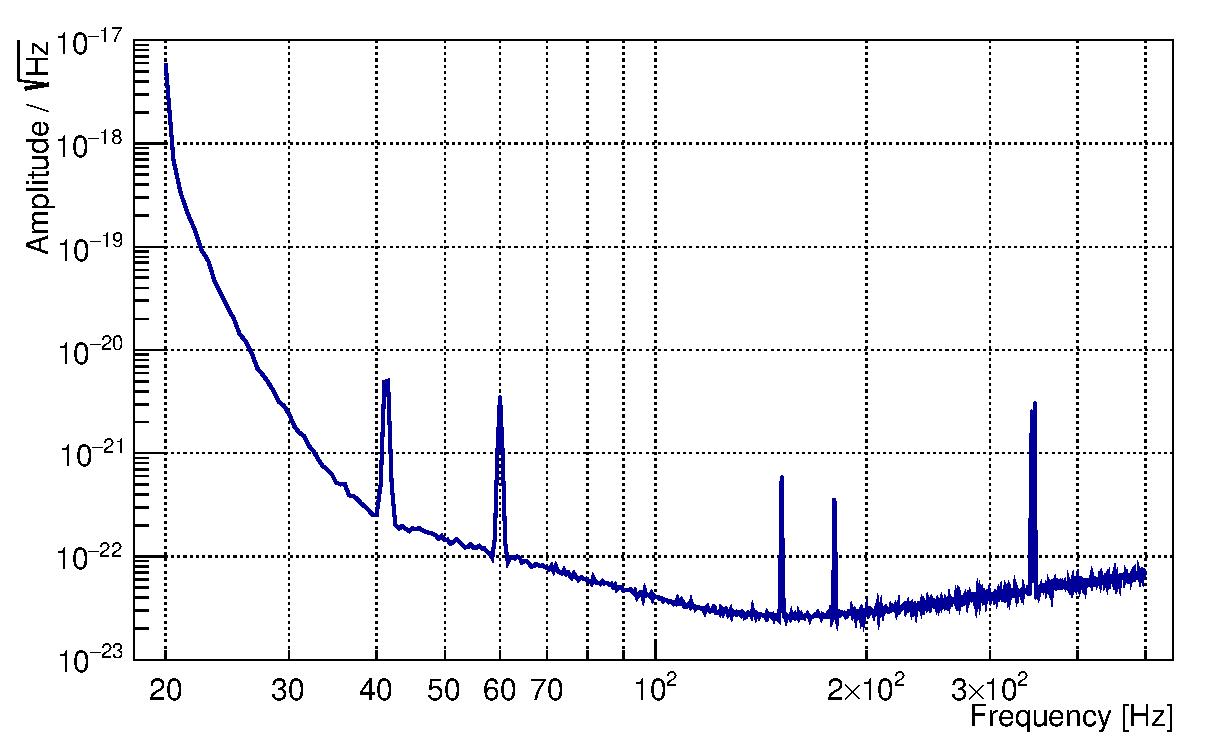
\epsfig{width=10cm, file=./figures/noise_asd.eps}
  \caption{Noise spectral density}
  \label{fig:noise_asd}
\end{figure}

\subsection{Detection efficiency} \label{sec:characterization:efficiency}

\subsection{Parameter recovery} \label{sec:characterization:parameter}

